\documentclass[beamer]{standalone}

\begin{document}
	\begin{frame}
		\color{blue}\centering\Huge{\textbf{Accelerazione}}	
	\end{frame}
	
	\begin{frame}{{Accelerazione}}
		\centering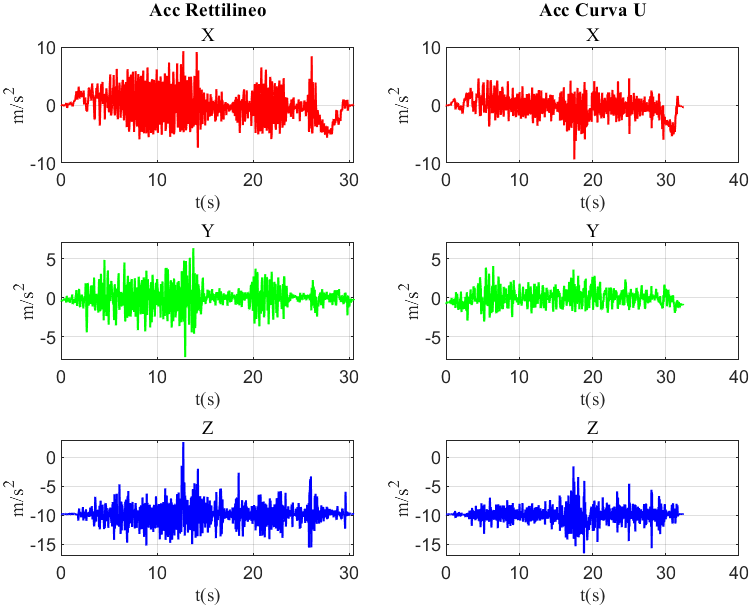
\includegraphics[height=.8\textheight]{figure/Acc/Acc}
	\end{frame}
	
	\begin{frame}{{Media}}
		\centering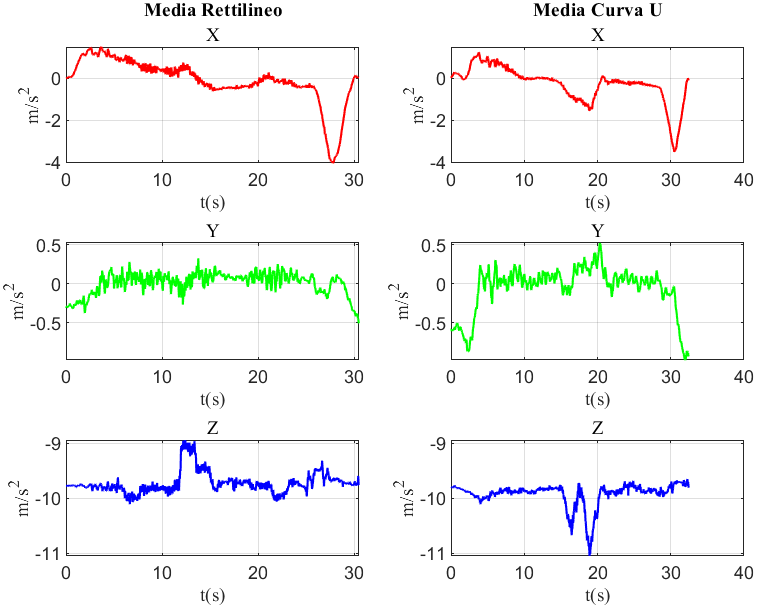
\includegraphics[height=.8\textheight]{figure/Acc/Media}
	\end{frame}
	
%	\begin{frame}{{Media Rettificata}}
%		\centering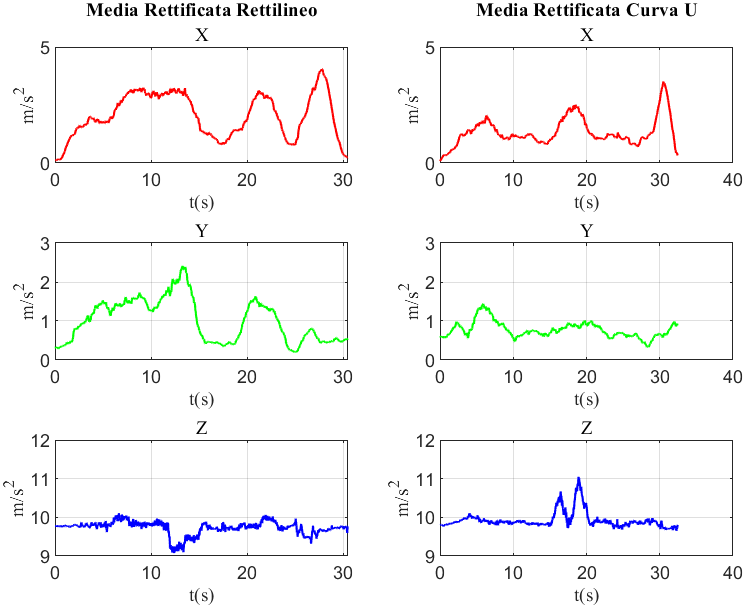
\includegraphics[height=.8\textheight]{figure/Acc/Media Rettificata}
%	\end{frame}

	\begin{frame}{{Varianza}}
		\centering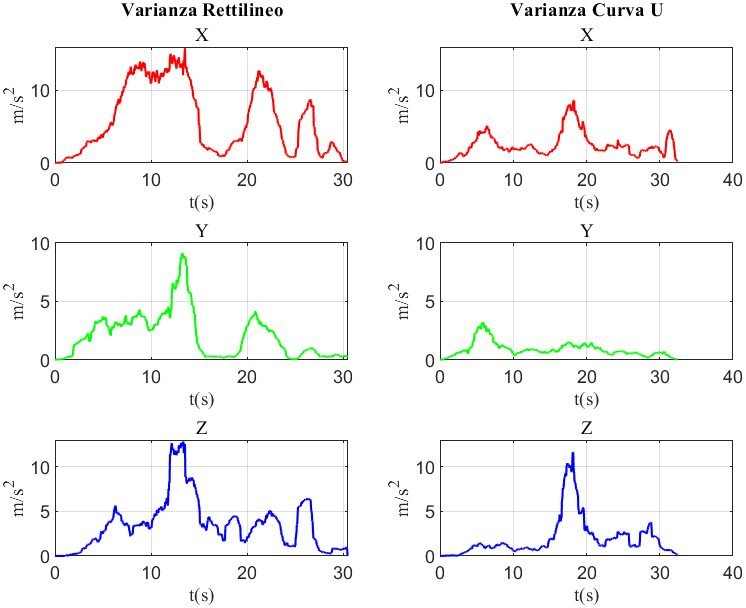
\includegraphics[height=.8\textheight]{figure/Acc/Varianza}
	\end{frame}
	
%	\begin{frame}{{Deviazione Standard}}
%		\centering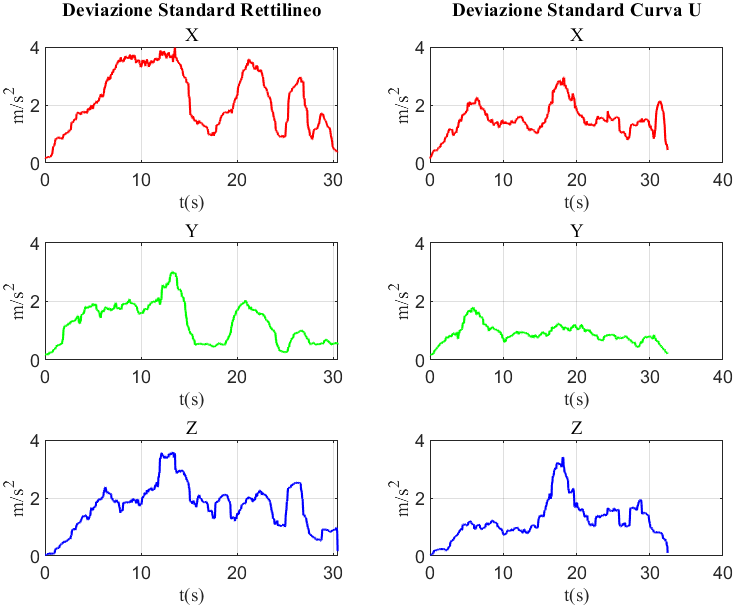
\includegraphics[height=.8\textheight]{figure/Acc/Deviazione Standard}
%	\end{frame}
%	
%	\begin{frame}{{Scarto Quadratico Medio}}
%		\centering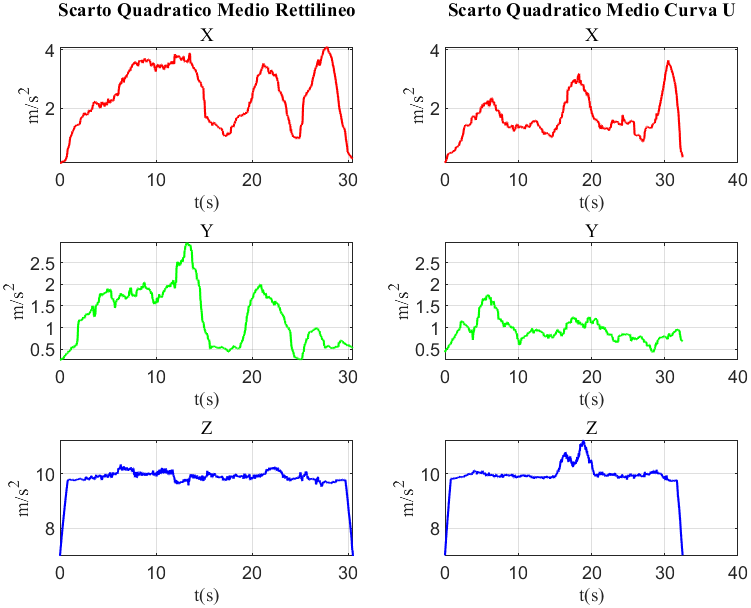
\includegraphics[height=.8\textheight]{figure/Acc/Scarto Quadratico Medio}
%	\end{frame}
	
	\begin{frame}{{Max}}
		\centering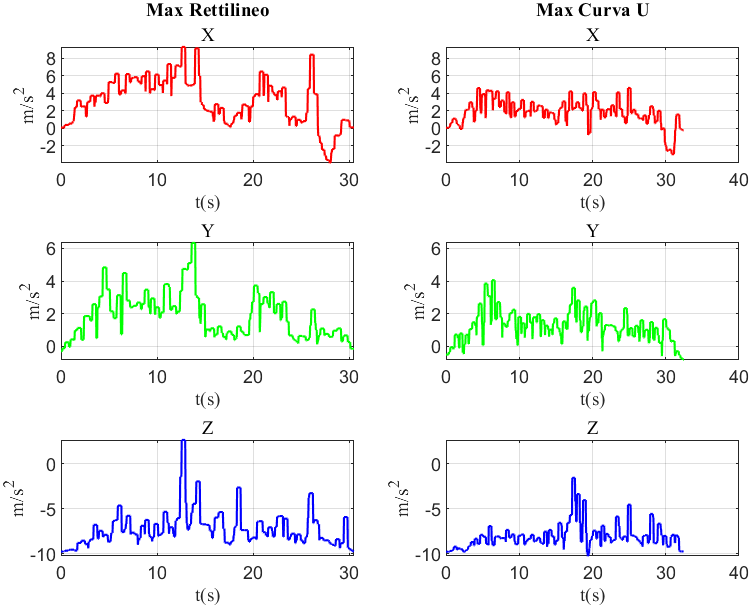
\includegraphics[height=.8\textheight]{figure/Acc/Max}
	\end{frame}
	
%	\begin{frame}{{Min}}
%		\centering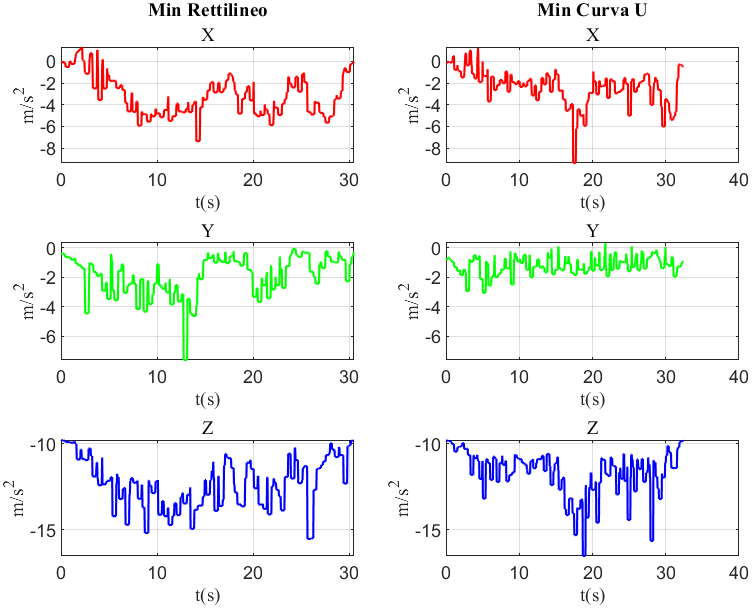
\includegraphics[height=.8\textheight]{figure/Acc/Min}
%	\end{frame}

	\begin{frame}{{Peak}}
		\centering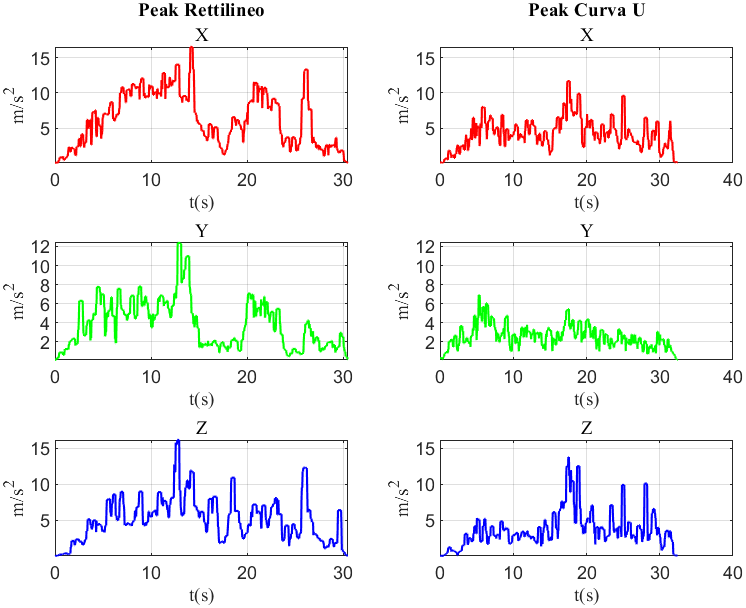
\includegraphics[height=.8\textheight]{figure/Acc/Peak}
	\end{frame}
	
%	\begin{frame}{{Kurtosi}}
%		\centering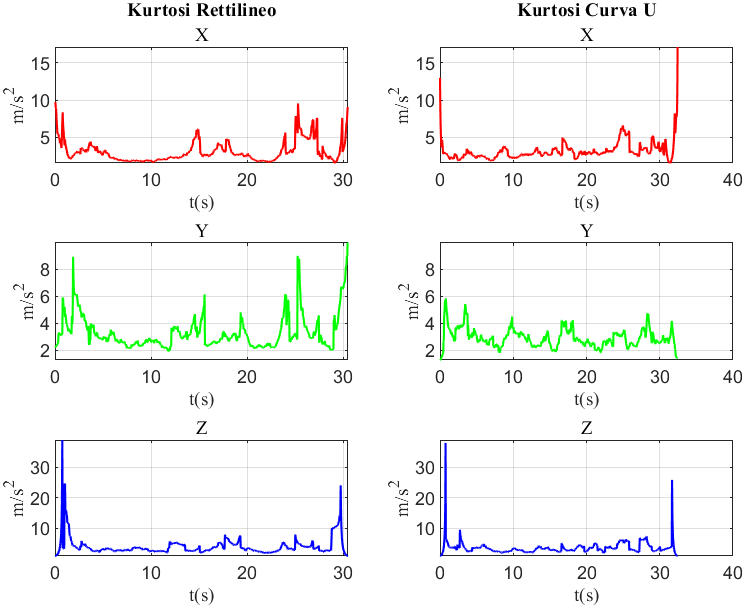
\includegraphics[height=.8\textheight]{figure/Acc/Kurtosi}
%	\end{frame}
%	
%	\begin{frame}{{Skewness}}
%		\centering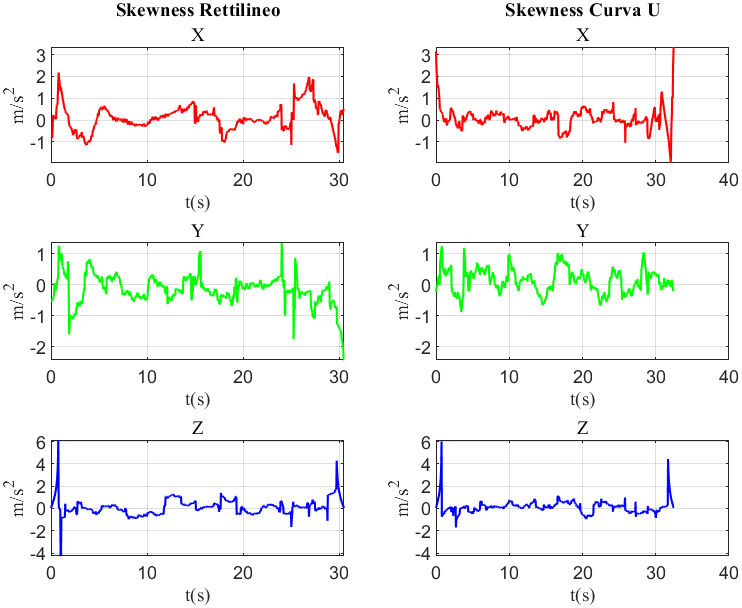
\includegraphics[height=.8\textheight]{figure/Acc/Skewness}
%	\end{frame}
%	
%	\begin{frame}{{Shape Factor}}
%		\centering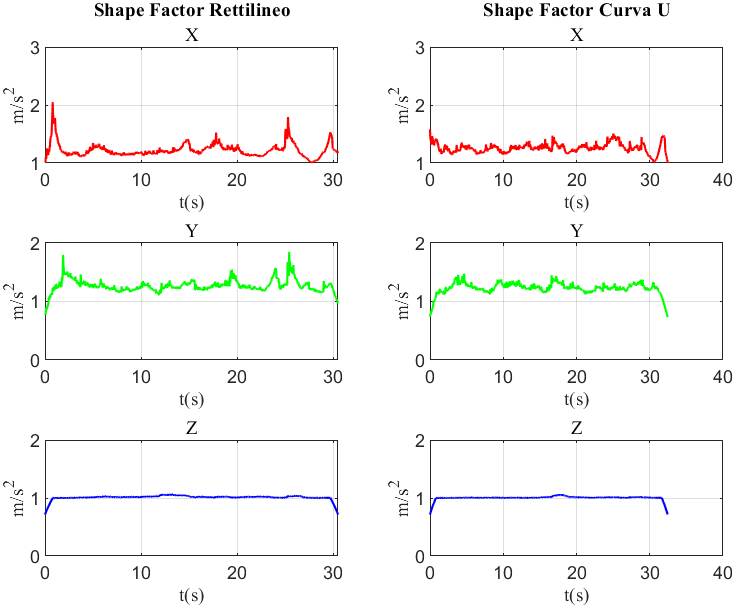
\includegraphics[height=.8\textheight]{figure/Acc/Shape Factor}
%	\end{frame}
%	
%	\begin{frame}{{Crest Factor}}
%		\centering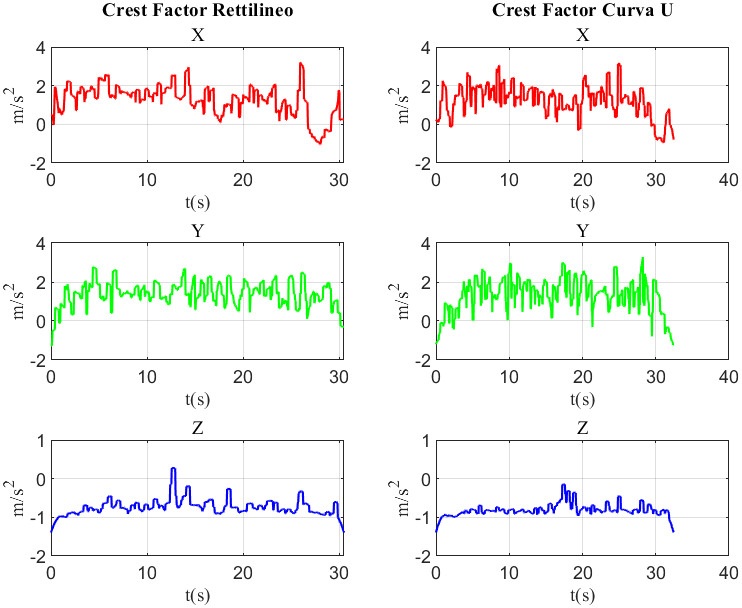
\includegraphics[height=.8\textheight]{figure/Acc/Crest Factor}
%	\end{frame}
%	
%	\begin{frame}{{Impulse Factor}}
%		\centering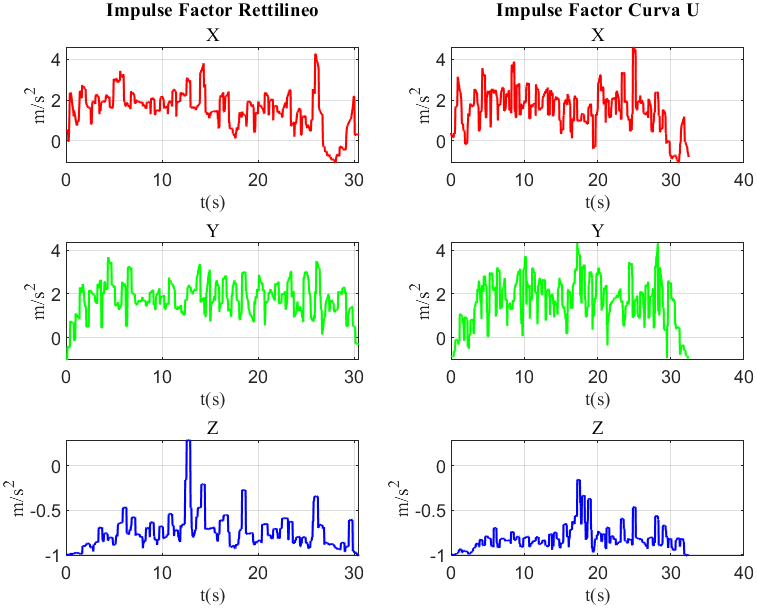
\includegraphics[height=.8\textheight]{figure/Acc/Impulse Factor}
%	\end{frame}
%	
%	\begin{frame}{{Margin Factor}}
%		\centering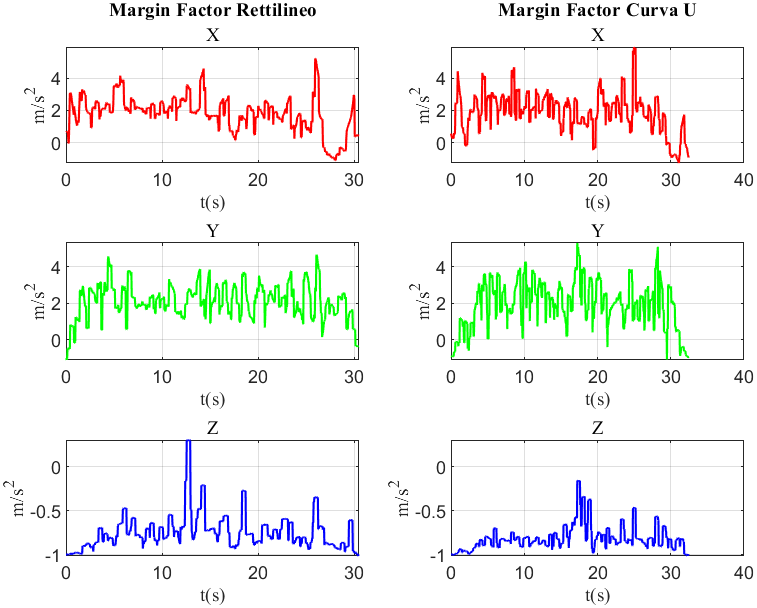
\includegraphics[height=.8\textheight]{figure/Acc/Margin Factor}
%	\end{frame}
	
%	\begin{frame}{{Trasformata}}
%		\centering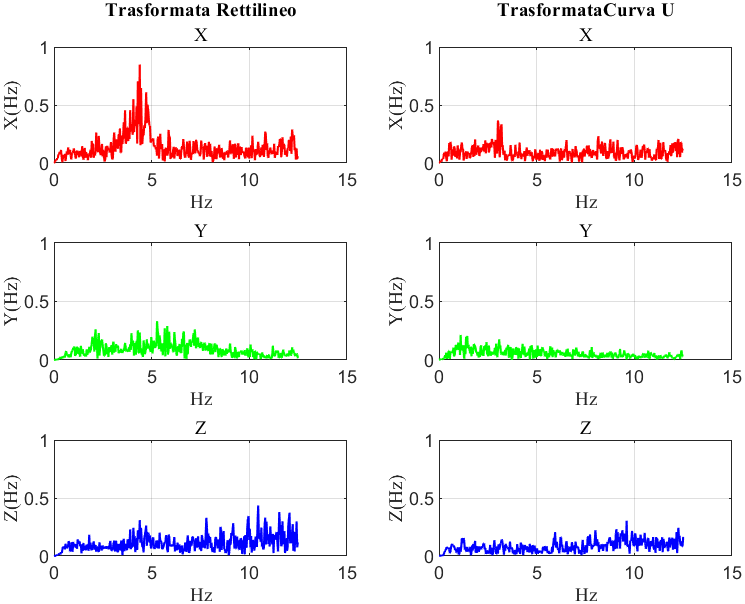
\includegraphics[height=.8\textheight]{figure/Acc/Trasformata/Trasformata}
%	\end{frame}
%
%	\begin{frame}{{Spettro}}
%		\centering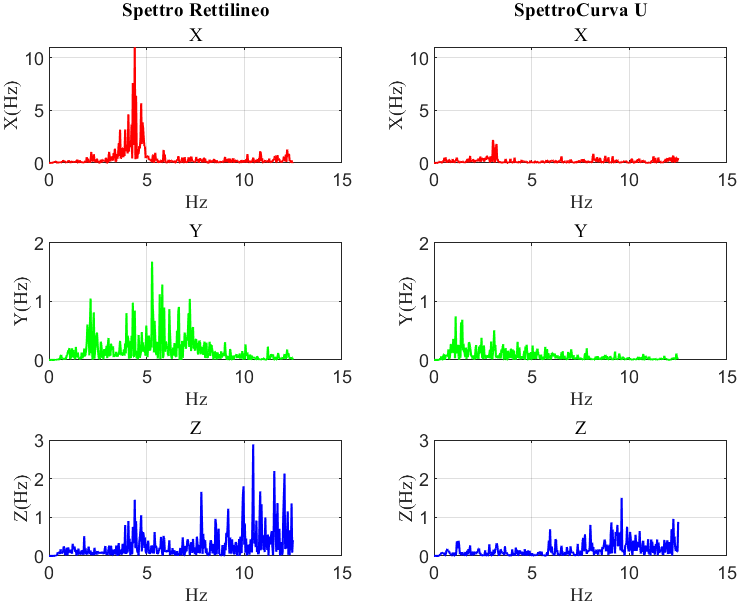
\includegraphics[height=.8\textheight]{figure/Acc/Trasformata/Spettro}
%	\end{frame}
%	
%	\begin{frame}
%		\color{blue}\centering\huge{\textbf{Trasformata Accelerazione}}
%	\end{frame}
%	
%	\begin{frame}{{Ampiezza Media X}}					
%		\centering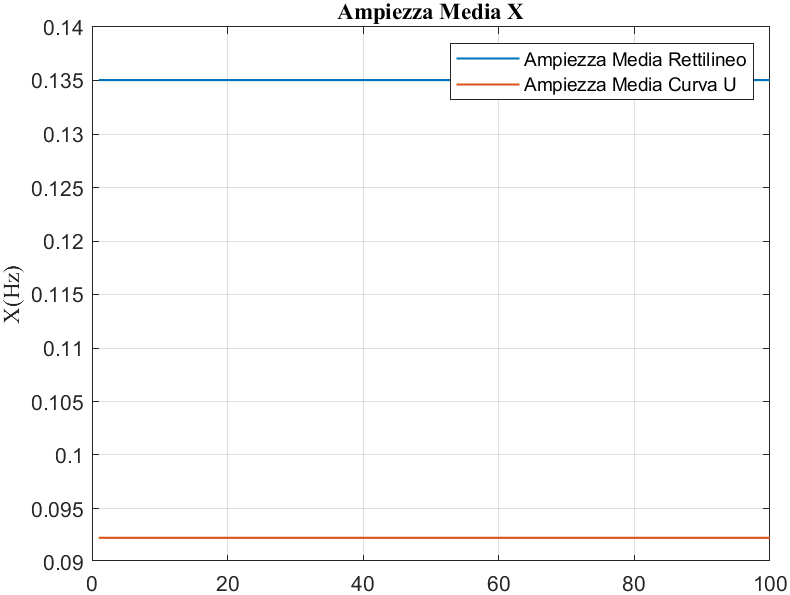
\includegraphics[height=.8\textheight]{figure/Acc/Trasformata/Ampiezza MediaX}
%	\end{frame}
%
%	\begin{frame}{{Ampiezza Media Y}}					
%		\centering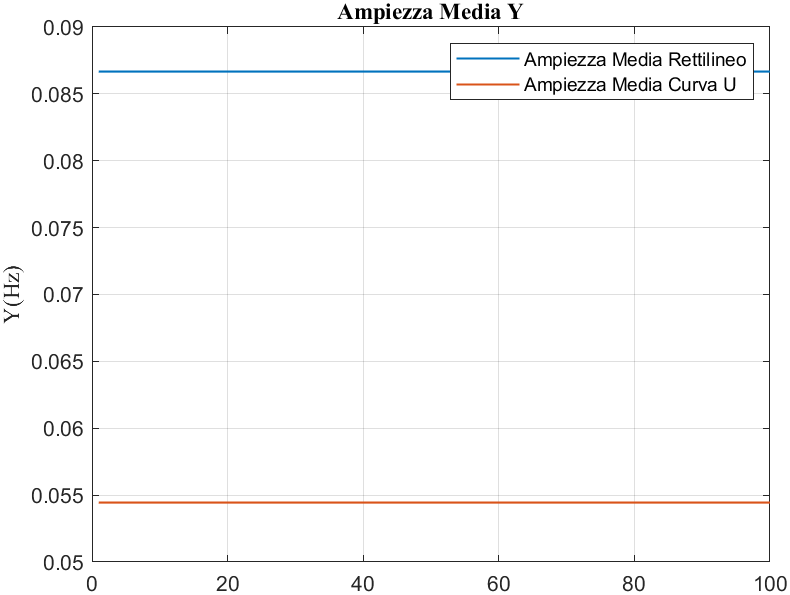
\includegraphics[height=.8\textheight]{figure/Acc/Trasformata/Ampiezza MediaY}
%	\end{frame}
%	
%	\begin{frame}{{Ampiezza Media Z}}					
%		\centering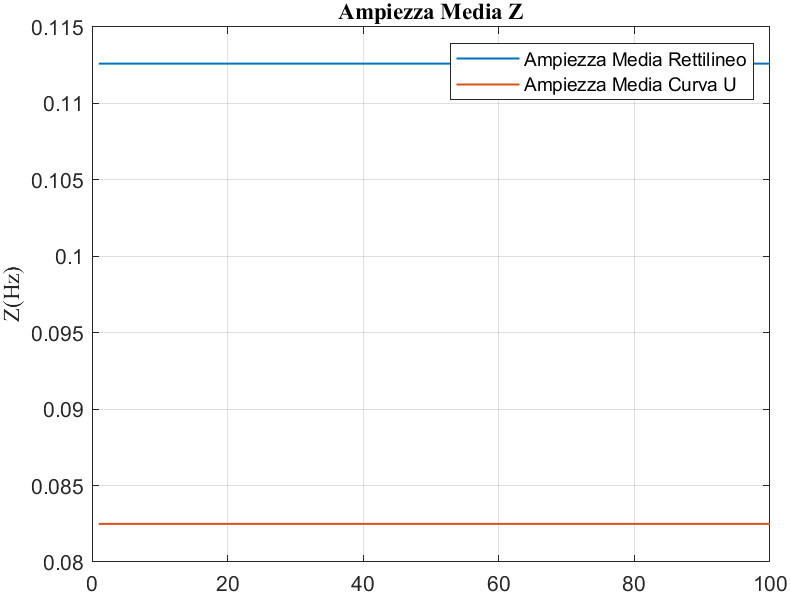
\includegraphics[height=.8\textheight]{figure/Acc/Trasformata/Ampiezza MediaZ}
%	\end{frame}
%	
%	\begin{frame}{{Frequency Centroid X}}
%		\centering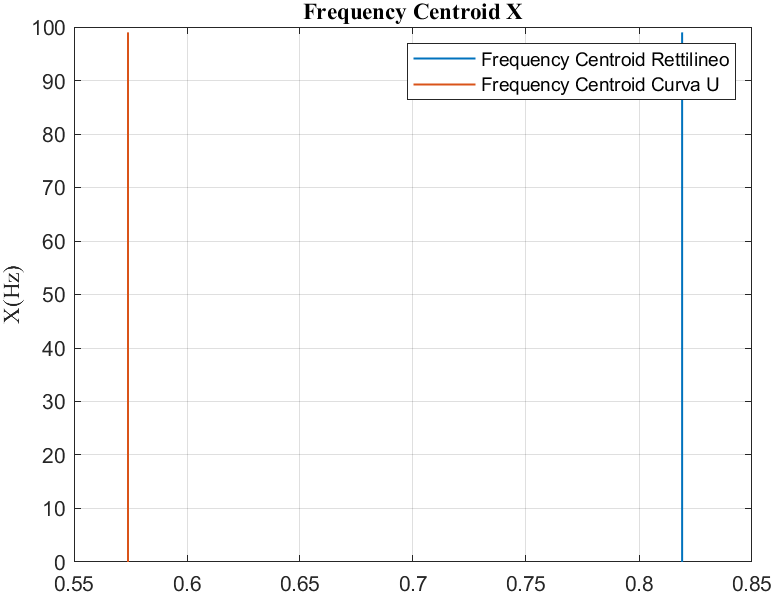
\includegraphics[height=.8\textheight]{figure/Acc/Trasformata/Frequency CentroidX}
%	\end{frame}
%
%	\begin{frame}{{Frequency Centroid Y}}
%		\centering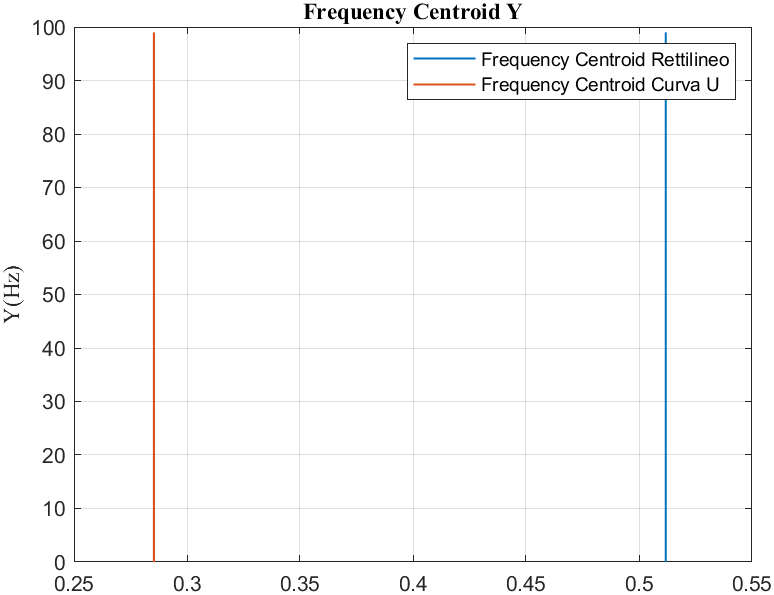
\includegraphics[height=.8\textheight]{figure/Acc/Trasformata/Frequency CentroidY}
%	\end{frame}
%	
%	\begin{frame}{{Frequency Centroid Z}}
%		\centering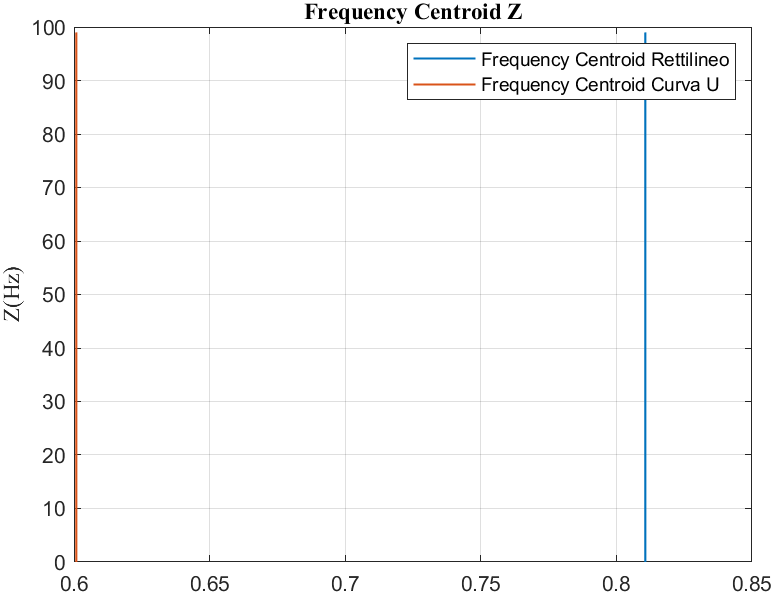
\includegraphics[height=.8\textheight]{figure/Acc/Trasformata/Frequency CentroidZ}
%	\end{frame}
%	
%	\begin{frame}{{Frequency Variance X}}
%		\centering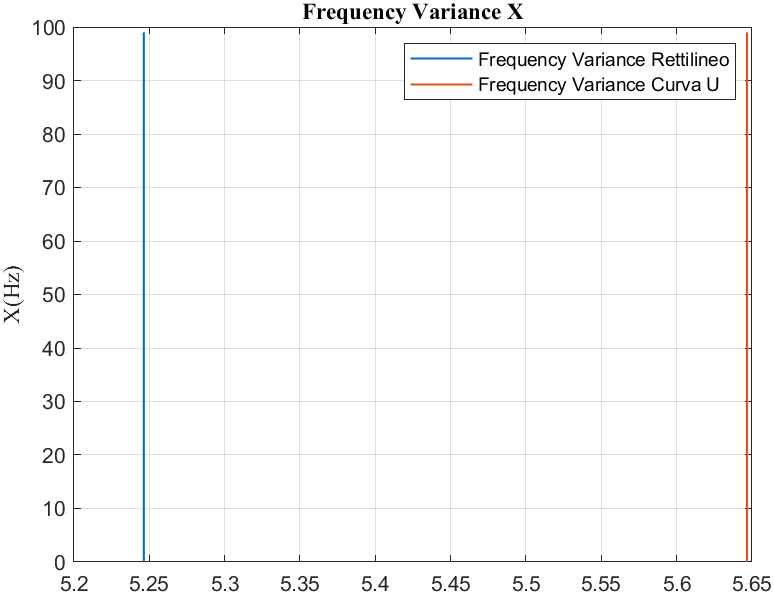
\includegraphics[height=.8\textheight]{figure/Acc/Trasformata/Frequency VarianceX}
%	\end{frame}
%	
%	\begin{frame}{{Frequency Variance Y}}
%		\centering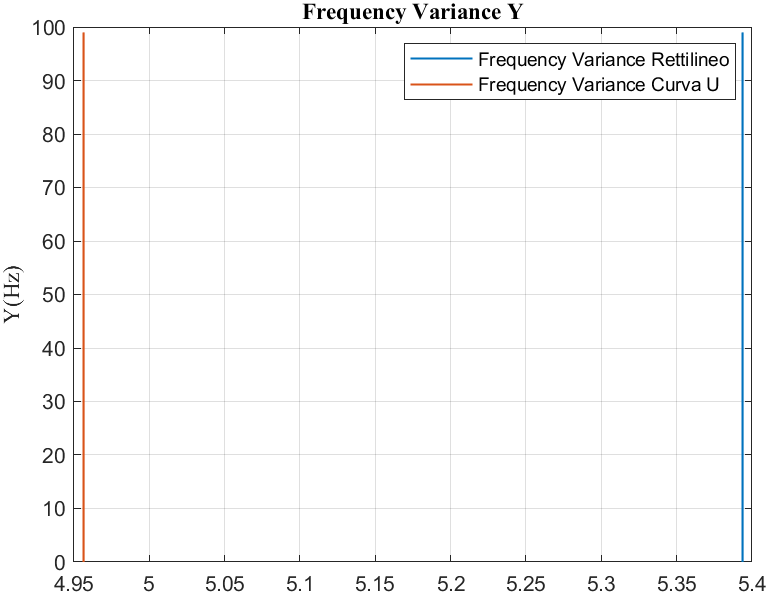
\includegraphics[height=.8\textheight]{figure/Acc/Trasformata/Frequency VarianceY}
%	\end{frame}
%	
%	\begin{frame}{{Frequency Variance Z}}
%		\centering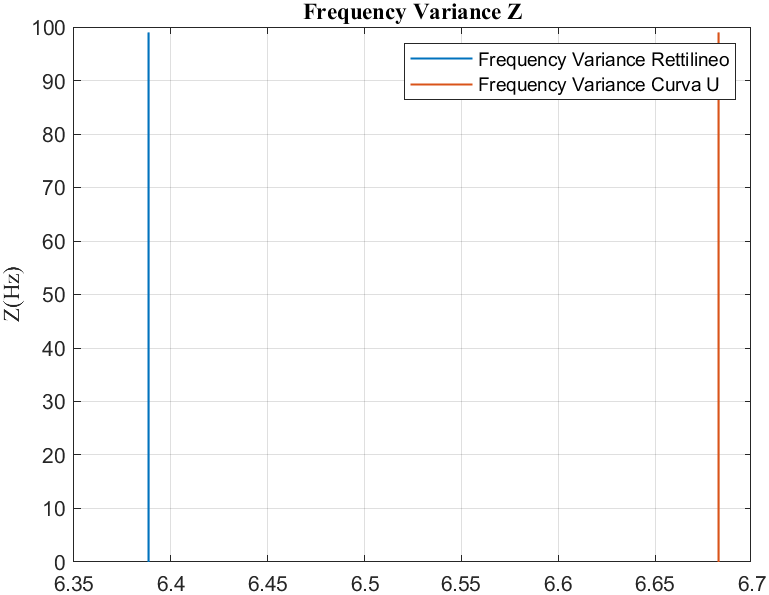
\includegraphics[height=.8\textheight]{figure/Acc/Trasformata/Frequency VarianceZ}
%	\end{frame}
%	
%	\begin{frame}
%		\color{blue}\centering\huge{\textbf{Spettro Accelerazione}}
%	\end{frame}
%	
%	\begin{frame}{{Spectral EntropyX}}
%		\centering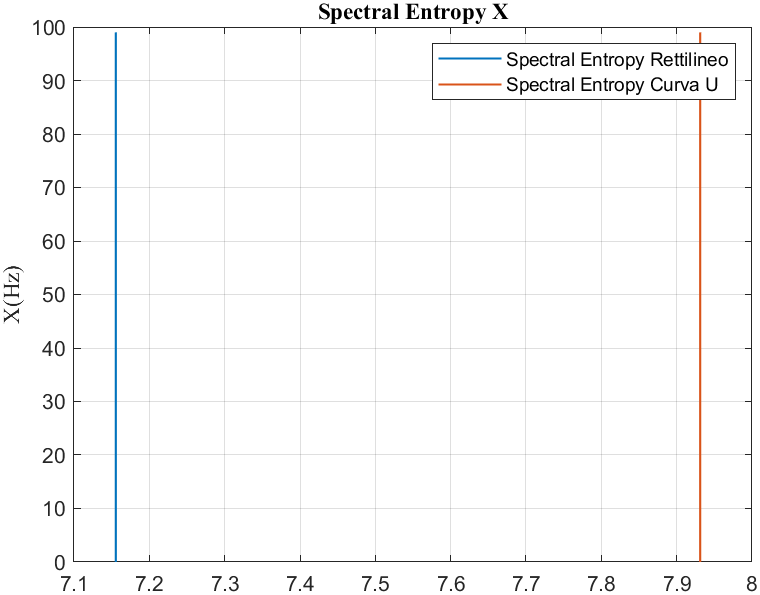
\includegraphics[height=.8\textheight]{figure/Acc/Trasformata/Spectral EntropyX}
%	\end{frame}
%	
%	\begin{frame}{{Spectral EntropyY}}
%		\centering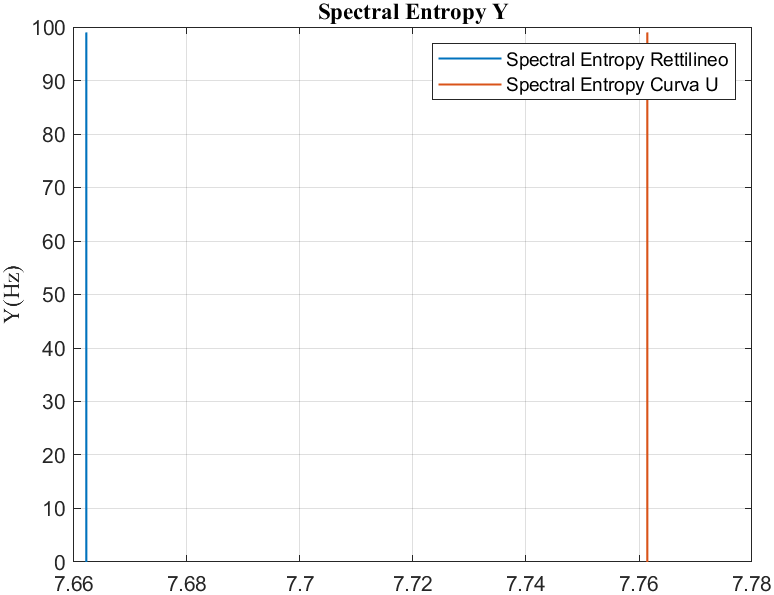
\includegraphics[height=.8\textheight]{figure/Acc/Trasformata/Spectral EntropyY}
%	\end{frame}
%	
%	\begin{frame}{{Spectral EntropyZ}}
%		\centering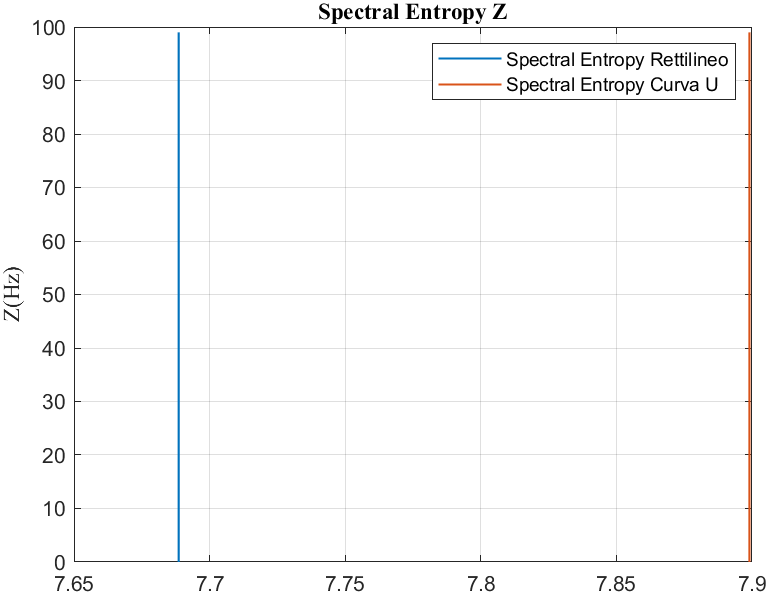
\includegraphics[height=.8\textheight]{figure/Acc/Trasformata/Spectral EntropyZ}
%	\end{frame}
	
\end{document}